\section{Regret Bound Comparison with Previous Work}
\label{app: comparison tables}

\begin{table}[H]
  \centering
  % --------- Table n ----------
  \caption{Regret for model-free learning in stochastic MDPs
           (only showing $T$ dependence). ``Toy 3-arm'' is defined in
           \pref{thm:lower bound}. The two bounds in the same cell correspond to the cases with on-policy and off-policy estimation. }   \label{tab: sto}
  % --- your first tabular ---
  \vspace*{-5pt}
  \hspace*{-25pt}
  \begin{tabular}{ |c|c|c|c|c| }
    \hline
    Algorithm & Bilinear or BE & \makecell{\{Bilinear or BE or Coverable\}\\ + Bellman Complete + On-Policy}& Toy 3-arm & Exploration Mechanism \\ \hline
    \makecell{\cite{du2021bilinear} \\ \cite{jin2021bellman} \\ \cite{xie2022role}} & $T^{\frac{2}{3}}/T^{\frac{2}{3}}$
      & $\sqrt{T}$ & $\sqrt{T}$ & optimism \\ \hline
    \cite{foster2024model} & $T^{\frac{3}{4}}/T^{\frac{5}{6}}$
      & $T^{\frac{2}{3}}$ & $\sqrt{T}$ & information gain + optimism \\ \hline
    Ours & $T^{\frac{2}{3}}/T^{\frac{7}{9}}$ & $\sqrt{T}$ & 1
      & information gain \\ \hline
  \end{tabular}

  \vspace{1.5em}  % optional vertical gap

  % --------- Table n+1 ----------
  \captionof{table}{Regret for learning in hybrid MDPs (stochastic transition and adversarial reward). The model-free learning guarantees in \cite{liu2025decision} and our work cannot handle general reward but rely on \pref{assum: known feature}. }
  \label{tab: adv}
  \vspace*{3pt}
  \hspace*{-23pt}
  % --- your second tabular ---
  \begin{tabular}{ |c|c|c|c|c|c| }
    \hline
    Algorithm & Bilinear & \makecell{ \{Bilinear or Coverable\}\\+ Bellman Complete + On-Policy} & Model-Free & Bandit Feedback & General Reward \\ \hline
    \cite{liu2025decision} & $\sqrt{T}/T^{\frac{2}{3}}$
      & $\sqrt{T}$ & \xmark & \cmark & \cmark \\ \hline
    \cite{liu2025decision} & $T^{\frac{3}{4}}/T^{\frac{5}{6}}$
      & -- &  \cmark & \xmark  & \xmark \\ \hline
    Ours & $T^{\frac{5}{6}}/T^{\frac{13}{15}}$
      & $T^{\frac{3}{4}}$ & \cmark & \cmark & \xmark  \\ \hline
  \end{tabular}
\end{table}




\section{Partitioning over $\calP\times \calR\times \Pi$ for hybrid MDPs}\label{app: illustrate}
\begin{figure}[H]
\centering
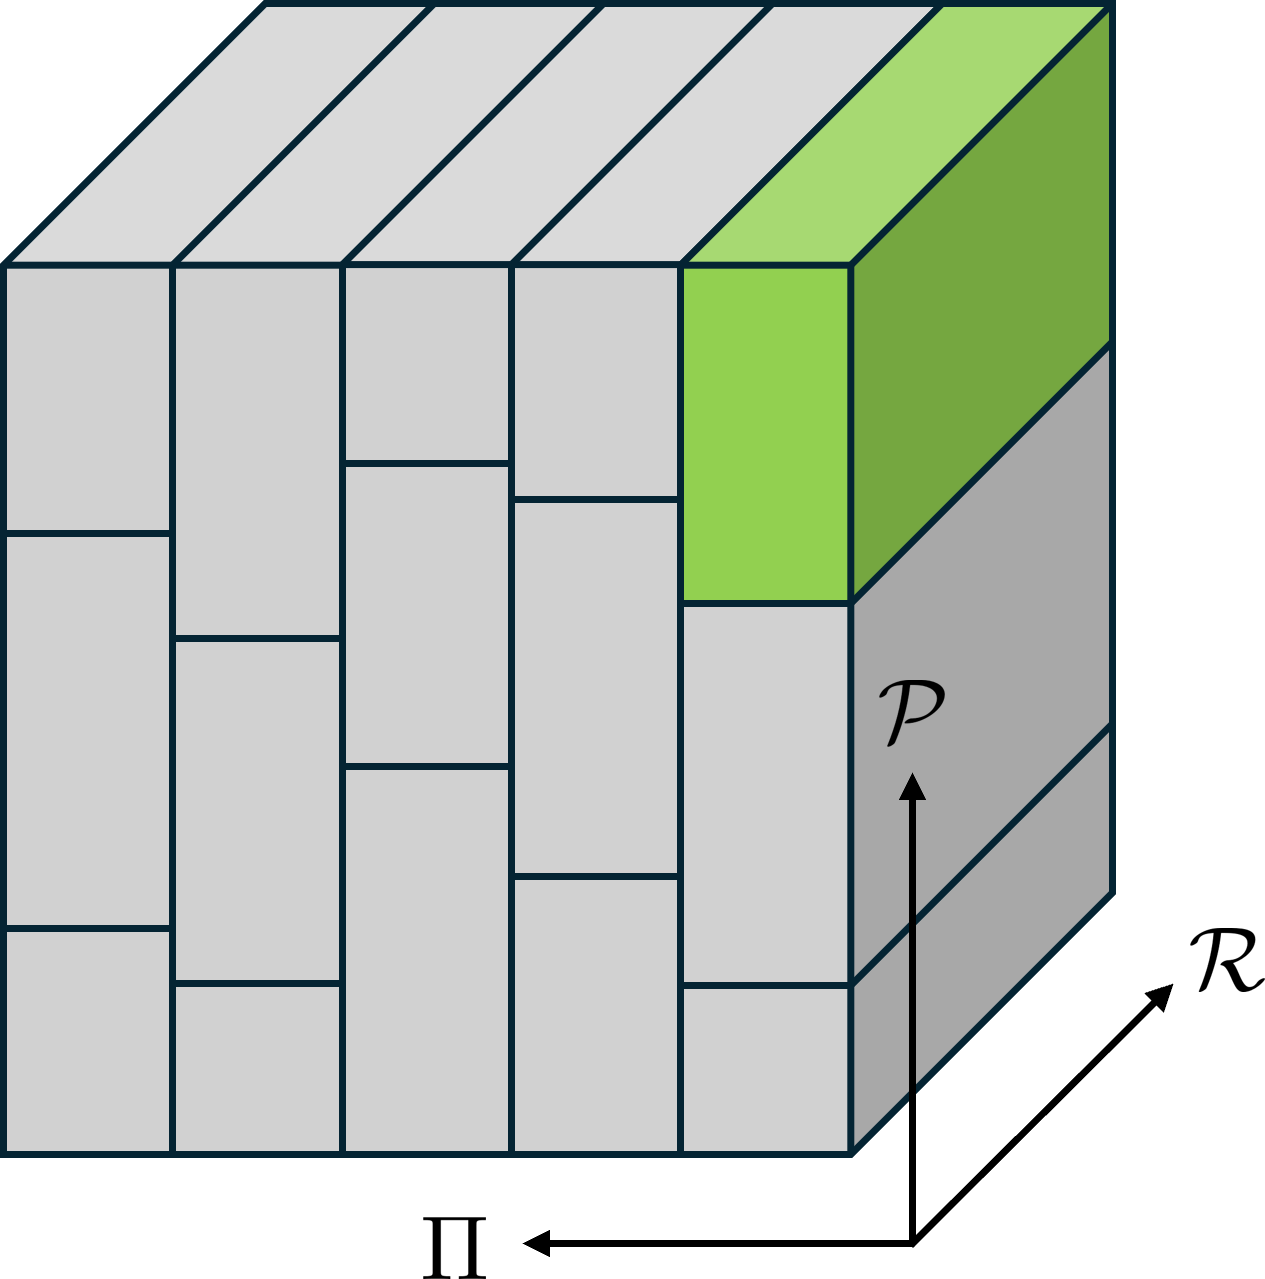
\includegraphics[width=0.3\textwidth]{Picture1.png}
\caption{Partitioning for hybrid MDPs}\label{fig: illustrate}
\end{figure}

\pref{fig: illustrate} illustrates the partition scheme over $\calM\times \Pi=\calP\times \calR\times \Pi$ described in \pref{assum: function approximation hybrid}. Each infoset $\phi$ (represented by the green block in \pref{fig: illustrate}) is associated with single policy $\pi_\phi$, a subset of transitions, and all reward functions. %Under a fixed policy $\pi$, transition $P$ and transition $P'$ should lie in the same $\phi$ if $Q^{\pi}(s,a; (P, R)) = Q^{\pi}(s,a; (P', R))$ for all $s,a,R$. 
As shown in \pref{fig: illustrate}, the partition over the $\calP$ space could be different for different $\pi$. 

